
%\documentclass[mathserif]{beamer}
\documentclass[handout]{beamer}
%\usetheme{Goettingen}
%\usetheme{Warsaw}
\usetheme{Singapore}



%\usetheme{Frankfurt}
%\usetheme{Copenhagen}
%\usetheme{Szeged}
%\usetheme{Montpellier}
%\usetheme{CambridgeUS}
%\usecolortheme{}
%\setbeamercovered{transparent}
\usepackage[english, activeacute]{babel}
\usepackage[utf8]{inputenc}
\usepackage{amsmath, amssymb}
\usepackage{dsfont}
\usepackage{graphics}
\usepackage{cases}
\usepackage{graphicx}
\usepackage{pgf}
\usepackage{epsfig}
\usepackage{amssymb}
\usepackage{multirow}	
\usepackage{amstext}
\usepackage[ruled,vlined,lined]{algorithm2e}
\usepackage{amsmath}
\usepackage{epic}
\usepackage{epsfig}
\usepackage{fontenc}
\usepackage{framed,color}
\usepackage{palatino, url, multicol}
%\algsetup{indent=2em}
\newcommand{\factorial}{\ensuremath{\mbox{\sc Factorial}}}
\newcommand{\BIGOP}[1]{\mathop{\mathchoice%
{\raise-0.22em\hbox{\huge $#1$}}%
{\raise-0.05em\hbox{\Large $#1$}}{\hbox{\large $#1$}}{#1}}}
\newcommand{\bigtimes}{\BIGOP{\times}}
\vspace{-0.5cm}
\title{Natural Language Processing \\ Large Language Models Usage and Evaluation Patterns}
\vspace{-0.5cm}
\author[Felipe Bravo Márquez]{\footnotesize
%\author{\footnotesize  
 \textcolor[rgb]{0.00,0.00,1.00}{Felipe Bravo-Marquez}} 
  
 

\date{\today}

\begin{document}
\begin{frame}
\titlepage


\end{frame}



\section{Introduction}
\begin{frame}{Introduction}
\begin{scriptsize}
\begin{itemize}
\item Since the inception of Large Language Models, various patterns of use and evaluation of this technology have emerged.
\item In this talk, we will try to organize these patterns and give a general overview of them.
\end{itemize}

 \begin{figure}[h]
        	
\includegraphics[scale = 0.2]{pics/Large-Language-Models.jpg}
        \end{figure}
Source: \url{https://www.masayume.it/img/masayume/Large-Language-Models.jpg}
\end{scriptsize}
\end{frame}



\begin{frame}{Recap: What is an LLM}
\begin{scriptsize}
\begin{itemize}
\item  An autoregressive language model trained with a Transformer neural network on a large corpus (hundreds of bullions of tokens) and a large parameter space (billions) to predict the next word.
\item It is usually later aligned to work as a user assistant using techniques such as Reinforcement Learning From Human Feedback  \cite{ouyang2022training} or supervised fine-tuning.
\item Some are private (access via API or web browser): Google Bard, ChatGPT, etc.
\item Others are open (model's weights can be downloaded): Llama, LLama2, Falcon, etc.
\end{itemize}
\end{scriptsize}
\end{frame}


\begin{frame}{Talk Overview}
\begin{scriptsize}

\begin{columns}[t]
\column{0.5\textwidth}
\begin{block}{Usage Patterns}
\begin{enumerate}
\item Fixed-knowledge Assistant
\item knowledge-augmented Assistant
\item Applications with LLMs in the middle
\item Agents
\end{enumerate}
\end{block}

\column{0.5\textwidth}
\begin{block}{Evaluation Patterns}
\begin{itemize}
\item MTBench
\item LLM Arena
\end{itemize}
\end{block}

\end{columns}

\end{scriptsize}
\end{frame}









% \url{https://ai.meta.com/llama/get-started/?trk=feed_main-feed-card_reshare_feed-article-content}.

\section{Prompting}

\begin{frame}{Prompting}
\begin{scriptsize}
\begin{itemize}
\item Prompt Engineering 
\item Chain of thought Prompting
\end{itemize}
\end{scriptsize}
\end{frame}


\section{Vector Databases}

\begin{frame}{Vector Databases}
\begin{scriptsize}
\begin{itemize}
\item Idea incorporate domain-scpefific knowledge not included during training.
\item Rely on a Vector Database embed queries, retrieve relevant documents, append them into the prompt \cite{lewis2021retrievalaugmented}.

\item \url{https://www.infoworld.com/article/3709912/vector-databases-in-llms-and-search.html}
\item \url{https://learn.deeplearning.ai/vector-databases-embeddings-applications/lesson/1/introduction}
\item \url{https://stackoverflow.blog/2023/10/09/from-prototype-to-production-vector-databases-in-generative-ai-applications/}
\end{itemize}
\end{scriptsize}

    \begin{figure}[h]
        	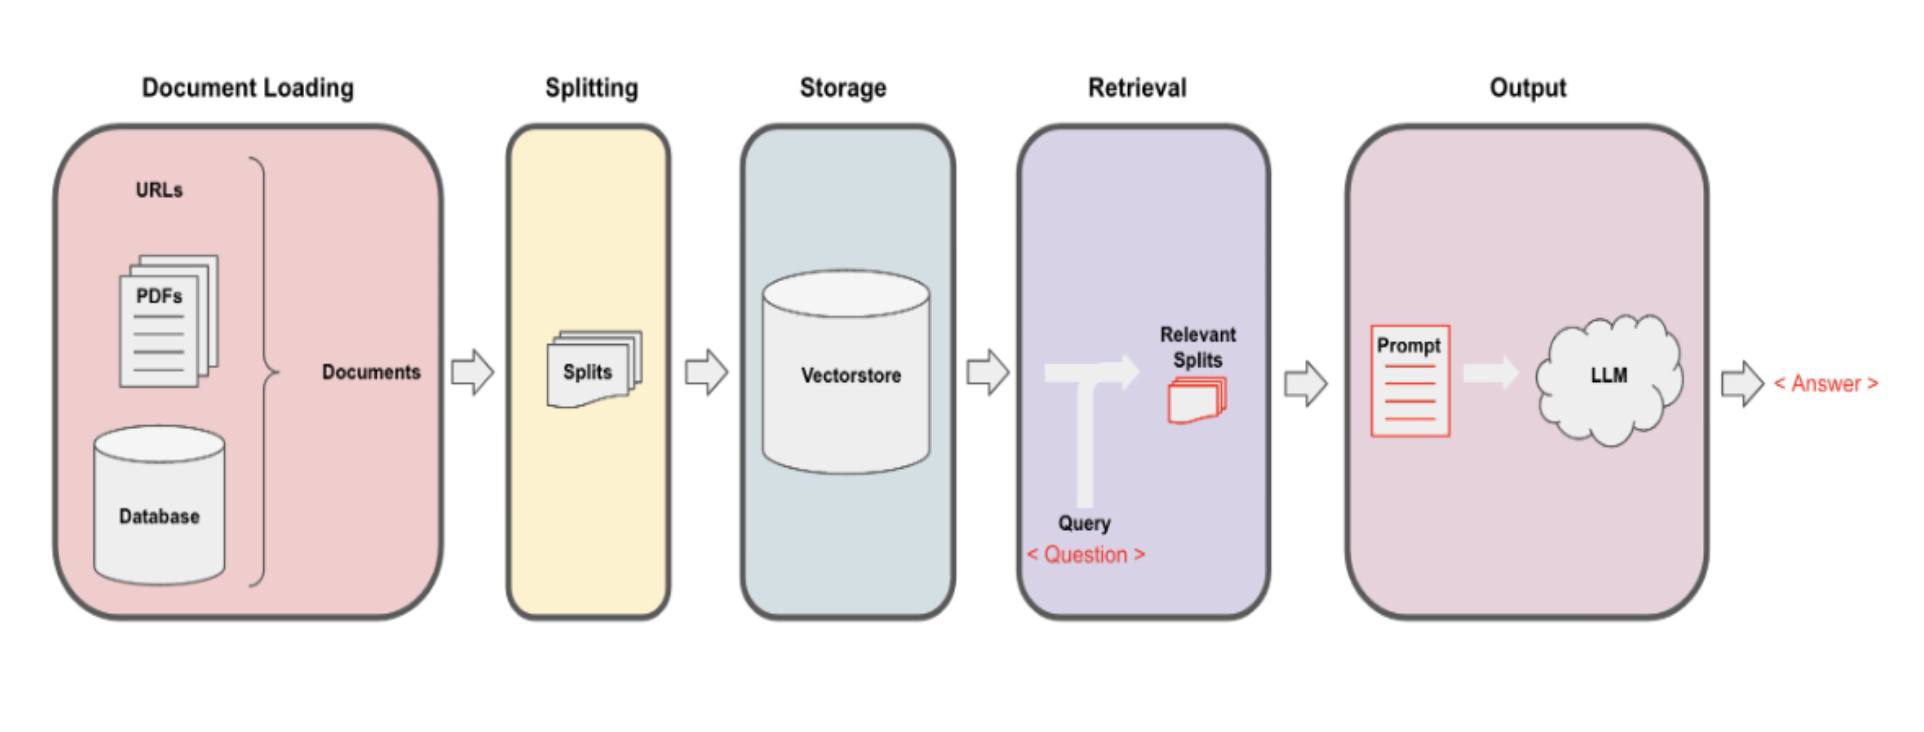
\includegraphics[scale = 0.4]{pics/vectordatabase.png}
        \end{figure}  


\end{frame}




\section{Fine-Tuning}

\begin{frame}{Instruction Fine-Tuning}
\begin{scriptsize}
\begin{itemize}
\item Paid Fine-Tuning (GPT-4??)
\item Alpaca, Vicuna, Llama, Llama2
\item https://blog.gopenai.com/paper-review-qlora-efficient-finetuning-of-quantized-llms-a3c857cd0cca
\end{itemize}
\end{scriptsize}
\end{frame}

\begin{frame}{Datasets for Instruction Fine-Tuning}
\begin{scriptsize}
\begin{itemize}
\item Standford Alpaca Dataset (Vicuna)
\item ShareGPT (Alpaca)
\item Dolly-15K
\item Orca Dataset
\end{itemize}
\end{scriptsize}
\end{frame}

\begin{frame}{Parameter Efficient Fine Tuning}
\begin{scriptsize}
\begin{itemize}
\item Lora, QLora
\item https://blog.gopenai.com/paper-review-qlora-efficient-finetuning-of-quantized-llms-a3c857cd0cca
\end{itemize}
\end{scriptsize}
\end{frame}

\begin{frame}{Token-Incrementation}
\begin{scriptsize}
\begin{itemize}
\item Lora, QLora
\item https://blog.gopenai.com/paper-review-qlora-efficient-finetuning-of-quantized-llms-a3c857cd0cca
\end{itemize}
\end{scriptsize}
\end{frame}

\section{Evaluation}
\begin{frame}{LLMBench and LLm Arena}
\begin{scriptsize}
\begin{itemize}
\item MT-bench (categories)
\item HuggingFace Open LLM Leaderboard
\item LLM Arena
\end{itemize}
\end{scriptsize}
\end{frame}



\section{Agents}

\begin{frame}{LangChain and Agents}
%https://arxiv.org/pdf/2304.03442.pdf
%https://bootcamp.uxdesign.cc/a-comprehensive-and-hands-on-guide-to-autonomous-agents-with-gpt-b58d54724d50
\begin{scriptsize}
\begin{itemize}
\item Bla
\end{itemize}
\end{scriptsize}
\end{frame}



\begin{frame}
\frametitle{Questions?}
%\vspace{1.5cm}
\begin{center}\LARGE Thanks for your Attention!\\ \end{center}



\end{frame}

\begin{frame}[allowframebreaks]\scriptsize
\frametitle{References}
\bibliography{bio}
\bibliographystyle{apalike}
%\bibliographystyle{flexbib}
\end{frame}  


%%%%%%%%%%%%%%%%%%%%%%%%%%%

\end{document}
